\subsection{Messverfahren}
\paragraph{Messung von Silber}
Für die Messung der Halbwertszeit von aktiviertem Silber wird eine Geiger-Müller-Zählrohrspannung zwischen \(\qty{500}{\volt}\) und \(\qty{550}{\volt}\) am Betriebsgerät eingestellt. Zunächst wird die Untergrundzählrate bestimmt, um diese später von den Messwerten abziehen zu können. Dazu wird die Torzeit \(t\) auf \(t=\qty{10}{\s}\) eingestellt und \(50\) Messungen durchgeführt, sodass die Untergrundzählrate über einen Zeitraum von etwa acht Minuten erfasst wird. Die Torzeit ist die Dauer einer Einzelmessung, in der alle in dieser Zeit aufgenommenen Counts \(N\) addiert werden und somit letzlich die Messgröße \(\frac{N}{t}\) ausgegeben wird. 

Anschließend wird die eigentliche Silbermessung durchgeführt. Die Träger mit den Silberblechen werden zur Aktivierung für sieben Minuten in der Neutronenquelle platziert. Nach Beendigung der Aktivierung wird das Präparat schnellstmöglich an das Zählrohr gebracht und dort mit einem Aluminiumblech fixiert. Die Messung startet mit einer Torzeit von \(\qty{10}{\s}\) über eine Gesamtzeit von \(\qty{400}{\s}\) Dieser Zyklus wird insgesamt viermal wiederholt, um die statistische Unsicherheit zu reduzieren. Die vier Messreihen werden anschließend addiert und gemeinsam ausgewertet.

\paragraph{Messung von Indium}
Für die Messung der Halbwertszeit von aktiviertem Indium wird analog vorgegangen. Das Messintervall wird dabei auf \(\qty{120}{\s}\) eingestellt. Das aktivierte Indium-Präparat wird in der Halterung fixiert und über einen Zeitraum von etwa \(50\) Minuten gemessen. Auch hier wird zuvor die Untergrundzählrate bestimmt, wobei die Torzeit entsprechend angepasst wird. Da bei der Aktivierung von Indium neben dem Grundzustand auch ein metastabiler Zustand mit sehr kurzer Halbwertszeit gebildet wird, wird der erste Messpunkt für den Fit vernachlässigt, da dieser vom eigentlichen Zerfall der betrachteten Isotope abweicht.
\vfill
\subsection{Messprotokoll}
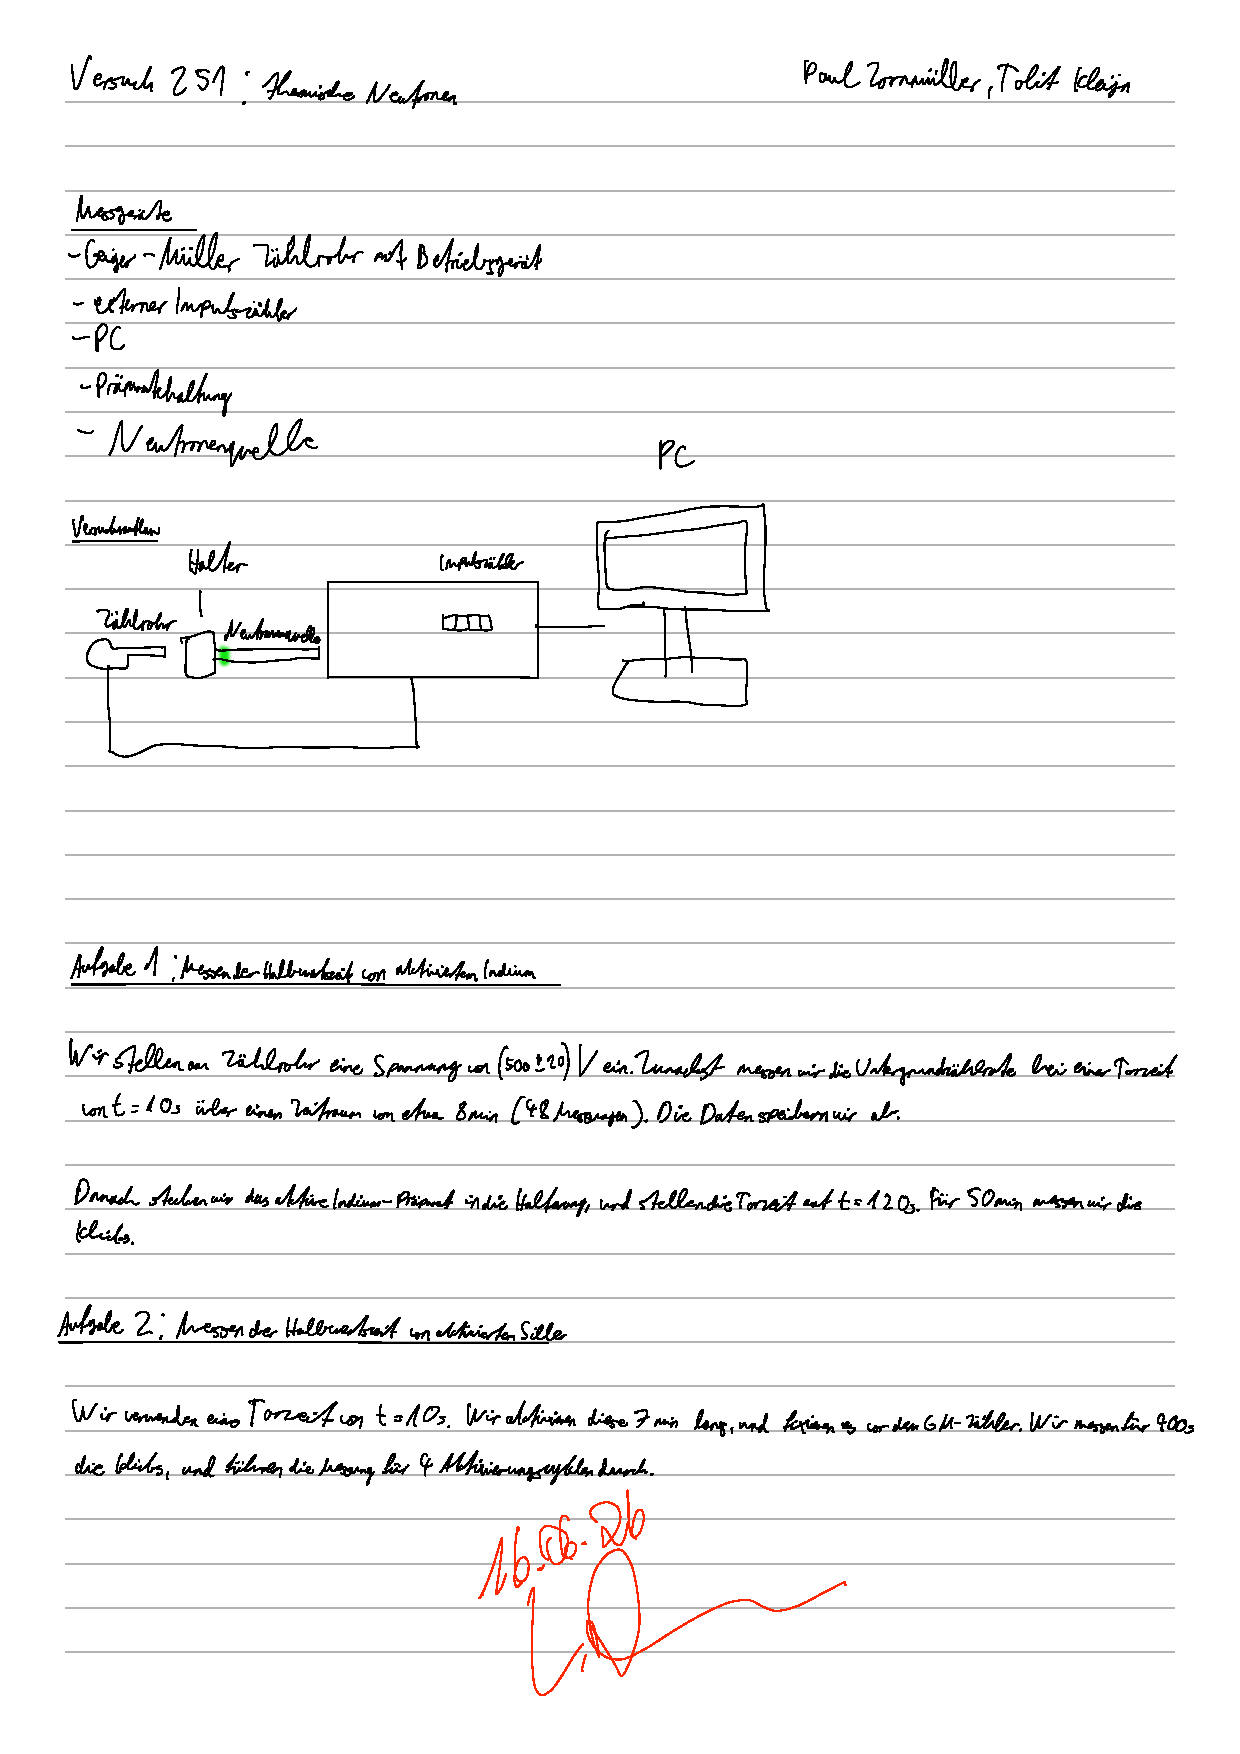
\includepdf[pages=-]{./images/252.pdf}
% heibox.uni-heidelberg.de/d/a48f9d7b91264990a16e/
